\documentclass[a4paper,12pt]{article}

\usepackage[utf8]{inputenc}
\usepackage{multirow,array}
\usepackage{graphicx}
\usepackage{a4wide}
\usepackage{longtable}
\newcommand{\HRule}{\rule{\linewidth}{1mm}}

\begin{document}


%
%  TITLE
%

\begin{titlepage}

\begin{center}
\huge An easy way to access files\\ in Gamma Mesh Format
\HRule \\
\medskip
{\Huge \bfseries The libMeshb library} \\
\HRule
\end{center}

\vfill

\begin{figure}[htbp]
\begin{center}
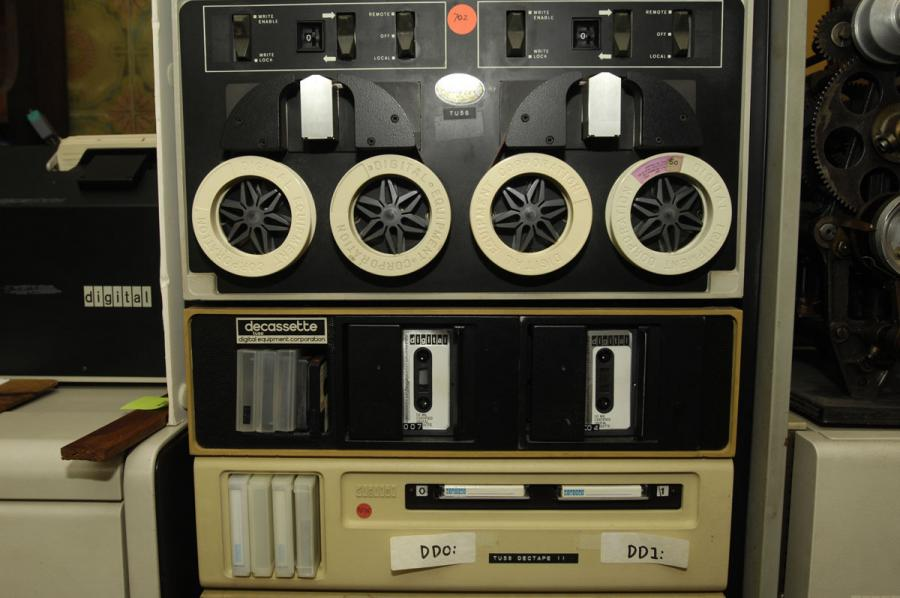
\includegraphics[width=14cm]{tape.jpeg}
\end{center}
\end{figure}

\vfill

\begin{flushright}
\Large Lo\"ic MAR\'ECHAL / INRIA, Gamma Project\\
<<<<<<< HEAD
<<<<<<< HEAD
\Large November 2018 \\
\normalsize Document v1.83 \\
\normalsize Library v7.33
=======
\Large December 2018 \\
\normalsize Document v1.90 \\
\normalsize Library v7.40
>>>>>>> release/V1.4
=======
\Large March 2019 \\
\normalsize Document v1.91 \\
\normalsize Library v7.50
>>>>>>> release/RELEASE
\end{flushright}

\end{titlepage}

\clearpage

\setcounter{tocdepth}{2}
\tableofcontents
\vfill

\footnotesize{Cover pictures: A variety of magnetic tape drives from the 1970s including the famous DECtapes.}
\normalsize

\clearpage


%
%  1 / INTRODUCTION
%

\section{Introduction}

\subsection{What is the Gamma Mesh Format ?}
<<<<<<< HEAD
The Gamma Mesh Format (GMF) and the associated library \emph{libMeshb} provide programmers of simulation and meshing softwares with an easy way to store their meshes and physical solutions.
=======
The Gamma Mesh Format (GMF) and the associated library \emph{libMeshb} provide programmers of simulation and meshing software with an easy way to store their meshes and physical solutions.
>>>>>>> release/V1.4

The GMF features more than 90 kinds of data types, ranging from vertex to polyhedron or normal vectors to matrix solution fields.

The \emph{libMeshb} provides a convenient way to move data between those files, via keyword tags, and the user's own structures.


\subsection{An evolving keyword based format}
The GMF is a keyword based file format, meaning that a mesh file consists of a list of keywords, each followed by its data. No keyword is mandatory and a file may contain any combination of them. Furthermore, new keywords may be added while keeping upward and backward compatibility.

It means that older files can be accessed by newer version of the library and vice versa.


\subsection{A comprehensive C library}
The \emph{libMeshb} provides programmers with a comprehensive set of commands and keywords covering most common operations on many different kinds of mesh or physical solution related data.

Reading, writing and querying files is easily done by calling a couple of commands which are provided in an ANSI C file ``libmeshb7.c'' and a header file ``libmeshb7.h''. All is needed is compiling those files along with the calling software.

Fortran APIs are also available: ``libmeshb7.ins'' for F77 and F90.


\subsection{ASCII vs. Binary}
GMF files can be stored in ASCII or binary format (differentiated with \emph{.mesh} or \emph{.meshb} extensions).

This choice is transparent from a user's point of view and a routine reading GMF files will work on both kinds of storage.
The library determining the right access method depending on the file extension.

It is advised to use ASCII for debugging purpose only when a file needs to be hand-written or checked by a human eye. Otherwise, when performance, compactness and portability are of concerns, binary is the way to go.


\subsubsection{Size does matter}
Binary files have a slightly smaller footprint than their ASCII counterparts (typically 30\% less). Not only does it save space on hard drives, but it allows for faster transfer as well.


\subsubsection{About performance}
Great care has been taken on performance issues when creating the \emph{libMeshb}. When dealing with binary files, reading and writing throughput will only be limited by the speed of the physical media where those files are located. Speed ranging from 20 MB/s to 60 MB/s can be achieved with hard drives and 10 MB/s or 100 MB/s with fast ethernet and gigabit ethernet networks, respectively.

The \emph{libMeshb} performs very poorly in ASCII mode, which is more processor bound rather than hard-drive bound. Don't expect more than 5 or 10 MB/s throughput.

\subsubsection{Compatibility issue: little vs. big endian}
When it comes to binary storage, the compatibility problem posed by endianness always comes to mind.

Some processors like PowerPc or SPARC are called big endian because of the way they store bytes within a word from most significant byte to the lowest.

The other ones, like i86 (Intel core2, AMD opteron) or itanium, store bytes in the reverse order and are called little endian.

Consequently, a binary word written by a big endian processor cannot be read by a little endian one, and vice versa. This problem can be easily overcome by reversing bytes order when reading inverted data. The \emph{libMeshb} handles this compatibility issue via a control word that indicates which endian a mesh file was written in.

You may then use binary files as safely as ASCII ones.

\subsection{Mesh and Sol files}
For the sake of understanding, different extensions must be given to files containing mesh related keywords \emph{.mesh} or \emph{.meshb}, and files containing physical solution keywords \emph{.sol} or \emph{.solb}.

\subsection{File versions}
Over the years, the library had to adapt to ever-increasing system capabilities, henceforth, modification to the binary file format had to be done. As of today, there are three revisions of the meshb format:
\medskip

\begin{tabular}{|r|r|r|r|}
\hline
Version & Size of integers & Size of reals & Maximum size of file \\
\hline
1 & 32 bits & 32 bits & 2 Gigabytes \\
\hline
2 & 32 bits & 64 bits & 2 Gigabytes \\
\hline
3 & 32 bits & 64 bits & 8 Exa Bytes \\
\hline
4 & 64 bits & 64 bits & 8 Exa Bytes \\
\hline
\end{tabular}
\medskip

Although the \emph{libMeshb} still handles versions 1 and 2 for the sake of compatibility, it is strongly advised to create version 3 or 4 files since most computers are now 64-bit capable.

A word of caution: great care must be taken when setting the library's arguments type. Regardless of the file version, some arguments are mandatory 32-bit integers like the open mode tag, mesh dimension or the file version. Even in "full 64 bits" version 4 mesh file format, only the number of lines given or set by the GmfSetKeyword() of GmfStatKeyword() commands and vertex indices used by elements field are using 64 bit integers.

The 64-bit integer data type used by the library is the \emph{int64\_t}, which is defined in the standard include file \emph{stdint.h}. In case your system is too old to support 64-bit pointers and integers, you may define \emph{int64\_t} as a regular 32-bit \emph{int}. The library will be aware of it and will still be able to handle version 1 or 2 files.


%
% 2 / QUICKSTART
%

\section{Quick start}

This section will guide you through three simple examples from which you may easily cut and paste to build your own code.

\subsection{Reading a file}

Let's start with reading an existing mesh file.

Reading a mesh is a two-step scheme:

\begin{enumerate}
\item opening and checking the file and allocating data structures according to its content
\item reading fields of interest (vertices, elements, etc.) and storing them in the previously allocated structures
\end{enumerate}

\subsubsection{Open, check and allocate a mesh}

Opening a mesh file is done via the GmfOpenMesh() command. It allows to check for file existence and whether it is of the required version and dimension.

\begin{tt}
\begin{verbatim}
int64_t MeshIndex;
int Version, Dimension;
MeshIndex = GmfOpenMesh("testcase.meshb", GmfRead, &Version, &Dimension );
\end{verbatim}
\end{tt}
\normalfont

Then, the presence and quantity of each item can be checked and memory allocated accordingly via the GmfStatKwd() command.

\begin{tt}
\begin{verbatim}
int NumberOfTriangles, (*TableOfTriangles)[4];

NumberOfTriangles = GmfStatKwd( MeshIndex, GmfTriangles );

if(NumberOfTriangles > 0)
   TableOfTriangles = malloc(NumberOfTriangles * 4 * sizeof(int));
\end{verbatim}
\end{tt}
\normalfont


\subsubsection{Example: reading vertices and triangles}

Reading each keyword data is done via two commands:

\begin{itemize}
\item GmfGotoKwd() to set the file index to the beginning of keyword data
\item GmfGetLin() to read one line of data
\end{itemize}

Let's say we would like to open a file, check if it contains vertices and quads, and read those fields into their respective tables:

\begin{tt}
\begin{verbatim}
int64_t idx;
int ver, dim, nbt, (*tt)[4], nbv, *rt;
float (*ct)[3];

/* Try to open the file and ensure its version is 1
   (single precision reals) and dimension is 3 */

idx = GmfOpenMesh("tri.meshb", GmfRead, &ver, &dim );

if( !idx || (ver != 1) || (dim != 3) )
   exit(1);

/* Read the number of vertices and triangles and allocate
   a triangle table (tt[nbt][4]) to store each triangle
   vertices and reference (hence the fourth integer).
   Two tables are allocated for the vertices:
   ct[nbv][3] to store the three coordinates
   rt[nbv] to store the references. */

nbv = GmfStatKwd( idx, GmfVertices );
nbt = GmfStatKwd( idx, GmfTriangles );

if( !nbv || !nbt )
   exit(1);

tt = malloc( nbt * 4 * sizeof(int) );
ct = malloc( nbv * 3 * sizeof(float) );
rt = malloc( nbv * sizeof(int) );

/* Move the file pointer to the begining of vertices data
   and start to loop over them. Then do likewise with triangles. */

GmfGotoKwd( idx, GmfVertices );

for(i=0;i<nbv;i++)
  GmfGetLin( idx, GmfVertices, &ct[i][0], &ct[i][1], &ct[i][2], &rt[i]);

GmfGotoKwd( idx, GmfTriangles );

for(i=0;i<nbt;i++)
  GmfGetLin( idx, GmfTriangles, &tt[i][0], &tt[i][1], &tt[i][2], &tt[i][3] );

GmfCloseMesh( idx );
\end{verbatim}
\end{tt}
\normalfont


\subsection{Writing a file}

Writing a mesh is also a two-step scheme:

\begin{enumerate}
\item creating an empty mesh file with the right version and dimension
\item writing every field (vertices, elements, etc.)
\end{enumerate}

\subsubsection{Creating and defining a mesh}

Mesh name, version and the dimension must be provided at creation time. Creating a mesh following version 1 (single precision real numbers) in three dimensions named testcase.meshb runs this way:

\begin{tt}
\begin{verbatim}
Meshindex = GmfOpenMesh( "testcase.meshb", GmfWrite, 1, 3 );
\end{verbatim}
\end{tt}
\normalfont

\subsubsection{Example: writing vertices and triangles}

Following the reading example, we would like to write back the data to a new file:

\begin{tt}
\begin{verbatim}
int64_t idx;
int ver, dim, nbt, (*tt)[4], nbv, *rt;
float (*ct)[3];

/* Try to create a three-dimensional, version 1
   (single precision reals) file */

idx = GmfOpenMesh("tri.meshb", GmfWrite, 1, 3 );

if( !idx )
   exit(1);

/* Setup a vertex field with nbv lines
   and loop over vertices to write them down.
   Note that this time, direct values are passed on
   GmfSetLin() instead of pointers. */

GmfSetKwd( idx, GmfVertices, nbv );

for(i=0;i<nbv;i++)
  GmfSetLin( idx, GmfVertices, ct[i][0], ct[i][1], ct[i][2], rt[i]);

GmfSetKwd( idx, GmfTriangles, nbt );

for(i=0;i<nbt;i++)
  GmfSetLin( idx, GmfTriangles, tt[i][0], tt[i][1], tt[i][2], tt[i][3] );

GmfCloseMesh( idx );
\end{verbatim}
\end{tt}
\normalfont


\subsection{Doing it all together}

In this last example, the file "quad.mesh" a three-dimensional mesh made of quads will be read, transformed into a triangulated one, which will be written as "tri.mesh":

\begin{tt}
\begin{verbatim}
int64_t InpMsh, OutMsh;
int i, nbv, nbq, ver, dim, *rt, (*qt)[5];
float (*ct)[3];

// Open and check the input quadrilateral mesh
InpMsh = GmfOpenMesh("quad.mesh", GmfRead, &ver, &dim);

if( !InpMsh || (ver != 1) || (dim != 3) )
  exit(1);

// Allocate vertices and quads tables
nbv = GmfStatKwd(InpMsh, GmfVertices);
ct = malloc(nbv * 3 * sizeof(float));
rt = malloc(nbv * sizeof(int));

nbq = GmfStatKwd(InpMsh, GmfQuadrilaterals);
qt = malloc(nbq * 5 * sizeof(int));

// Read vertices and quads then close the input file
GmfGotoKwd(InpMsh, GmfVertices);

for(i=0;i<nbv;i++)
  GmfGetLin(InpMsh, GmfVertices, &ct[i][0], &ct[i][1], &ct[i][2], &rt[i]);

GmfGotoKwd(InpMsh, GmfQuadrilaterals);

for(i=0;i<nbq;i++)
  GmfGetLin(InpMsh, GmfQuadrilaterals, &qt[i][0],
            &qt[i][1], &qt[i][2], &qt[i][3], &qt[i][4]);

GmfCloseMesh(InpMsh);

// Now create the output file.
// Each quad being split into two triangles.

if(!(OutMsh = GmfOpenMesh("tri.mesh", GmfWrite, ver, dim)))
  exit(1);

GmfSetKwd(OutMsh, GmfVertices, nbv);

for(i=0;i<nbv;i++)
  GmfSetLin(OutMsh, GmfVertices, ct[i][0], ct[i][1], ct[i][2], rt[i]);

GmfSetKwd(OutMsh, GmfTriangles, 2*nbq);

for(i=1;i<=nbq;i++)
{
  GmfSetLin(OutMsh, GmfTriangles, qt[i][0], qt[i][1], qt[i][2], qt[i][4]);
  GmfSetLin(OutMsh, GmfTriangles, qt[i][0], qt[i][2], qt[i][3], qt[i][4]);
}

GmfCloseMesh(OutMsh);
\end{verbatim}
\end{tt}
\normalfont


%
% 3 / COMMANDS
%

\newpage
\section{Commands}

\subsection{GmfOpenMesh}
Open a mesh file for reading or writing: in reading mode, it tries to open the file and returns some information about its content, in writing mode it creates an empty mesh file.

\subsubsection{Reading mode}
\begin{tt}
\begin{verbatim}
int64_t GmfOpenMesh( char *FileName,
                     int OpenMode,
                     int *Version,
                     int *Dimension );
\end{verbatim}
\end{tt}
\normalfont

\paragraph{FileName:}
this string must contain the path and the mesh name with its extension (meshes/my\_mesh.meshb).

\paragraph{OpenMode:}
must be set to GmfRead.

\paragraph{Version:}
will be set to the value read from the file, which may range from 1 to 3.

\begin{enumerate}
	\item real numbers in the whole file are written in single precision (32 bits)
	\item real numbers in the whole file are written in double precision (64 bits)
	\item same as 2 but file size may be greater than 2 GBytes.
\end{enumerate}

\paragraph{Dimension:}
will be set to the value read from the file, only dimensions 2 and 3 are supported.

\paragraph{Returns:}
Zero on failure or the open mesh index otherwise. This index should be properly stored since it must be provided to any further \emph{libMeshb} commands working on this file.

\paragraph{Example:} open a mesh file and print its version and dimension.

\begin{tt}
\begin{verbatim}
int64_t MeshIndex;
int Version, Dimension;

Meshindex = GmfOpenMesh("testcase.meshb", GmfRead, &Version, &Dimension );

if(MeshIndex)
    printf("Version = %d, Dimension = %d\n.", Version, Dimension);
else
    puts("This file cannot be opened.");
\end{verbatim}
\end{tt}
\normalfont


\subsubsection{Writing mode}
\begin{tt}
\begin{verbatim}
int64_t GmfOpenMesh( char *FileName,
                     int OpenMode,
                     int Version,
                     int Dimension );
\end{verbatim}
\end{tt}
\normalfont

\paragraph{FileName:}
this string must contain the path and the mesh name with its extension (meshes/my\_mesh.meshb).

\paragraph{OpenMode:}
must be set to GmfWrite.

\paragraph{Version:}
must be provided at file creation, see \emph{Reading mode} for version values.

\paragraph{Dimension:}
must be provided at file creation, only dimensions 2 and 3 are supported.

\paragraph{Returns:}
zero on failure or the open mesh index otherwise. This index should be properly stored since it must be provided to any further \emph{libMeshb} commands working on this file.

\paragraph{Example:} create a new three-dimensional mesh file storing double precision numbers.

\begin{tt}
\begin{verbatim}
Meshindex = GmfOpenMesh("newfile.meshb", GmfWrite, 2, 3 );
\end{verbatim}
\end{tt}
\normalfont


\subsection{GmfCloseMesh}
A mesh file must be properly closed in order to release any allocated memory and to write tailing information.

\begin{tt}
\begin{verbatim}
GmfCloseMesh( int64_t MeshIndex );
\end{verbatim}
\end{tt}
\normalfont

\paragraph{MeshIdx:}
the index returned by GmfOpenMesh() must be provided for the file to be closed.


\subsection{GmfStatKwd}
This command queries the mesh file for the presence of a given keyword and the number of associated lines.


\subsubsection{Getting information on a mesh keyword}

\begin{tt}
\begin{verbatim}
int GmfStatKwd( int64_t MeshIndex,
                int Keyword );
\end{verbatim}
\end{tt}
\normalfont

\paragraph{MeshIndex:} index of referenced mesh.

\paragraph{Keyword:} the keyword tag you are requesting information on (see section \ref{keywords} for a full list of available keywords).

\paragraph{Example:} check out and print the number of triangles in a mesh file.

\begin{tt}
\begin{verbatim}
int NumberOfTriangles;

NumberOfTriangles = GmfStatKwd( MeshIndex, GmfTriangles );

if(NumberOfTriangles)
    printf("This file contains %d triangles\n.", NumberOfTriangles);
else
    puts("This file does not contain any triangle.");
\end{verbatim}
\end{tt}
\normalfont

\subsubsection{Getting information on a solution keyword}
In this case, additional information will be provided: the number of fields per solution, the number of real numbers a solution line occupies and a table of solution types.

\begin{tt}
\begin{verbatim}
int64_t GmfStatKwd( int64_t MeshIndex,
                    int Keyword,
                    int *NumberOfTypes,
                    int *SizeOfSolution,
                    int *TableOfTypes );
\end{verbatim}
\end{tt}
\normalfont

\paragraph{MeshIndex:} index of referenced mesh.

\paragraph{Keyword:} the keyword tag you are requesting information on (see section \ref{keywords} for a full list of available keywords).

\paragraph{NumberOfTypes:} pointer to an integer, it will be set to the number of fields in the solution.

\paragraph{SizeOfSolution:} pointer to an integer, it will be set to the number of real numbers (float or double depending on the file version) used by a solution line for memory allocation purpose.

\paragraph{TableOfTypes:} pointer to a previously allocated table which will be filled with the type of each solution field.

\paragraph{Example:} check out and print the number of solutions and their kinds associated to vertices.

\begin{tt}
\begin{verbatim}
int NmbSol, NmbTypes, NmbReals, TypesTab[ GmfMaxTyp ];

NmbSol = GmfStatKwd( MeshIndex, NmbSol, &NmbTypes, &NmbReals, TypesTab );

if(NmbSol)
{
  printf("This file contains %d solutions at each vertex\n.", NmbSol);
  printf("Each solution contains %d fields:\n", NmbTypes);

  for(i=0; i<NmbTypes; i++)
  {
    switch(TypesTab[i])
    {
      case GmfSca    : printf("scalar,\n"); break;
      case GmfVec    : printf("vector of %d scalars,\n", dim); break;
      case GmfSymMat : printf("upper triangular part of a symetric \
                       %d x %d matrix,\n", dim, dim); break;
      case GmfMat    : printf("full %d x %d matrix,\n", dim, dim); break;
    }
  }
}
else
    puts("This file does not contain triangles.");
\end{verbatim}
\end{tt}
\normalfont


\subsection{GmfGotoKwd}
Prior to reading each line of a keyword with the GmfGetLin() command, the file position must be set to the beginning of its data with GmfGotoKwd(). Note that positioning the file mark is only needed when reading, not writing.

\begin{tt}
\begin{verbatim}
int GmfGotoKwd( int64_t MeshIndex, int Keyword );
\end{verbatim}
\end{tt}
\normalfont

\paragraph{MeshIdx:}
the index returned by GmfOpenMesh() must be provided.

\paragraph{KeyWord:} code of the keyword whose data are to be read.

\paragraph{Returns:} zero if this keyword is not present in the pointed file, one otherwise.


\subsection{GmfSetKwd}
Prior to writing each line of a keyword with the GmfSetLin() command, the keyword header should be written along with the number of lines.

\subsubsection{Writing a mesh keyword}

\begin{tt}
\begin{verbatim}
int GmfSetKwd( int64_t MeshIndex,
               int Keyword,
               int NumberOfLines );
\end{verbatim}
\end{tt}
\normalfont

\paragraph{MeshIdx:}
the index returned by GmfOpenMesh() must be provided.

\paragraph{KeyWord:} code of the keyword whose data are to be written.

\paragraph{NumberOfLines:} number of data lines which are to be written.

\paragraph{Returns:} zero if the data could not be written, and the number written lines otherwise.

\subsubsection{Writing a solution keyword}
When it comes to solution keywords, two extra arguments must be passed on: a table of solution types and its size.

\begin{tt}
\begin{verbatim}
int GmfSetKwd( int64_t MeshIndex,
               int Keyword,
               int NumberOfLines,
               int NumberOfTypes,
               int *TableOfTypes );
\end{verbatim}
\end{tt}
\normalfont

\paragraph{MeshIdx:}
the index returned by GmfOpenMesh() must be provided.

\paragraph{KeyWord:} code of the keyword whose data are to be written.

\paragraph{NumberOfLines:} number of data lines which are to be written.

\paragraph{NumberOfTypes:} the number of fields stored for each line of this solution. It sets the size of the following TableOfTypes containing each field type.

\paragraph{TableOfTypes:} pointer to a table of integers, each entry setting the type of each solution field: 1 for a scalar, 2 for a vector, 3 for symmetric matrix and 4 for a full matrix.

\paragraph{Returns:} zero if the data could not be written, and the number written lines otherwise.


\subsection{GmfGetLin}
GmfGetLin() is a variable argument command, it reads one line of data from the file and stores each item in the provided pointers to users' data structures.

\begin{tt}
\begin{verbatim}
int GmfGetLin( int64_t MeshIndex,
               int Keyword,
               arguments );
\end{verbatim}
\end{tt}
\normalfont

\paragraph{MeshIdx:}
the index returned by GmfOpenMesh() must be provided.

\paragraph{KeyWord:} code of the keyword whose line data is to be read.

\paragraph{arguments:} as many pointers to the required type of data as stated by the keyword definition (see section \ref{keywords}) should be provided.

\paragraph{Example:} reading a vertex in three-dimensional case. Caution: the right size of real numbers, float or double, should be provided according to the mesh file version.

\begin{tt}
\begin{verbatim}
int ref;
float xf, yf, zf;
double xd, yd, zd;

if(Version == 1)
    GmfGetLine(MeshIndex, GmfVertices, &xf, &yf, &zf, &ref);
else
    GmfGetLine(MeshIndex, GmfVertices, &xd, &yd, &zd, &ref);
\end{verbatim}
\end{tt}
\normalfont


\subsection{GmfSetLin}
This command works pretty much like GmfGetLin(), but arguments are given directly instead of pointers.

\begin{tt}
\begin{verbatim}
int GmfSetLin( int64_t MeshIndex,
               int Keyword,
               arguments );
\end{verbatim}
\end{tt}
\normalfont

\paragraph{MeshIdx:}
the index returned by GmfOpenMesh() must be provided.

\paragraph{KeyWord:} code of the keyword whose line of data is to be written.

\paragraph{arguments:} as many values of the required type of data as stated by the keyword definition (see section \ref{keywords}) should be provided.


\subsection{GmfGetBlock}
GmfGetBlock() is a variable argument command, it reads all the lines of data from the file and stores each item in the provided pointers to users' data structures. The user's data structure has to be fully described in order for the library to fill all the lines automatically.

\begin{tt}
\begin{verbatim}
int GmfGetBlock(int64_t MeshIndex, int Keyword, int64_t BeginLine, 
                int64_t EndLine, int MapType, void *RenumberingMap,
                void *Procedure, arguments...);
\end{verbatim}
\end{tt}
\normalfont

\paragraph{MeshIdx:}
the index returned by GmfOpenMesh() must be provided.

\paragraph{KeyWord:} code of the keyword whose lines of data are to be read.

\paragraph{BeginLine:} starting line in the mesh file, it enables partial reading for parallelism.

\paragraph{EndLine:} ending line in the mesh file.

\paragraph{MapType:} set the integer type (GmfInt or GmfLong) of the following renumbering table.

\paragraph{RenumberingMap:} pointer to a renumbering table that gives the position to store each mesh entity in the user's table (for example: give the old to new renumbering through a Hilbert curve).

\paragraph{Procedure:} pointer to an optional user's procedure that will be called in  parallel after each block has been read. If a procedure is given, a second pointer on users' data must be provided right after.

\paragraph{arguments:} for each type of data as stated by the keyword definition (see section \ref{keywords}), three arguments must be provided. First, the user's type of data in which the file's data will be stored (four kinds are available: GmfFloat, GmfDouble, GmfInt and GmfLong). Second, a pointer to the first line of this data type in the user's structure. Third, the same pointer but on the last line. The example below is more telling.

\clearpage
\paragraph{Example:} reading all vertices in three-dimensional case.

\begin{tt}
\begin{verbatim}
int ref[nv];
double x[nv], y[nv], z[nv];

GmfGetBlock(MeshIndex, GmfVertices, 1, nv, 0, NULL, NULL,
            GmfDouble,   &x[1],   &x[nv],
            GmfDouble,   &y[1],   &y[nv],
            GmfDouble,   &z[1],   &z[nv],
            GmfInt,    &ref[1], &ref[nv]);
\end{verbatim}
\end{tt}
\normalfont

\paragraph{Vector addresses:} In order to reduce the number of parameters, when dealing with high order polyhedra for example, you may concatenate a set of pointers into one base address and a size, a kind of address vector. The data will be loaded at consecutive addresses.

To indicate that the following begin and end set of pointers should be considered as a vector, you have to replace the GmfInt parameter by GmtIntVec followed by the size of the vector. Conversely, GmtLong, GmfFloat and GmfDouble can be replaced by GmfLongVec, GmfFloatVec and GmfDoubleVec in any keyword.

In this example, the first GmfGetBlock reading hexahedra may be replaced by the second one:

\begin{tt}
\begin{verbatim}
GmfGetBlock(MeshIndex, GmfVertices, 1, nh, 0, NULL, NULL,
            GmfInt, &HexIdx[1][0],   &HexIdx[nh][0],
            GmfInt, &HexIdx[1][1],   &HexIdx[nh][1],
            GmfInt, &HexIdx[1][2],   &HexIdx[nh][2],
            GmfInt, &HexIdx[1][3],   &HexIdx[nh][3],
            GmfInt, &HexIdx[1][4],   &HexIdx[nh][4],
            GmfInt, &HexIdx[1][5],   &HexIdx[nh][5],
            GmfInt, &HexIdx[1][6],   &HexIdx[nh][6],
            GmfInt, &HexIdx[1][7],   &HexIdx[nh][7],
            GmfInt, &HexRef[1],      &HexRef[nh]);

GmfGetBlock(MeshIndex, GmfVertices, 1, nh, 0, NULL, NULL,
            GmfIntVec, 8, &HexIdx[1],   &HexIdx[nh],
            GmfInt,       &HexRef[1],   &HexRef[nh]);

\end{verbatim}
\end{tt}
\normalfont

\paragraph{Arguments list vs arguments table:} In some situations, explicitly giving a long list of arguments to this procedure may be cumbersome as the C variable arguments call must be known and set at compile time. It is then impossible to automatically generate a reading call to a high order solution field with arbitrary order.
The solution id to provide data arguments (type, vector size, begin and ending pointers) through tables and not directly as procedure arguments.

To select this calling mode all you have to do is to pass "GmfArgTab" instead of the first user data type tag.
Then, the procedure expects four tables: one integer table containing the types, a second integer table containing the vector sizes (optional if only scalar data types are used) and the two following tables to store the pairs of first and last item pointers.

\begin{tt}
\begin{verbatim}
int   TypTab[2] = {GmfIntVec, GmfInt};
int   SizTab[2] = {8, 0};
void *BegTab[2] = {&HexIdx[ 1], &HexRef[ 1]};
void *EndTab[2] = {&HexIdx[nh], &HexIdx[nh]};

GmfGetBlock(MeshIndex, GmfVertices, 1, nh, 0, NULL, NULL,
            GmfArgTab, TypTab, SizTab, BegTab, EndTab);
\end{verbatim}
\end{tt}
\normalfont


\subsection{GmfSetBlock}
Works exactly as GmfGetBlock except that all lines are written, you cannot specify starting and ending lines in the file since concurrent writing is not supported for now. Note that you still need to set the keyword first with the help of GmfSetKwd() prior to writing the whole data lines with GmfSetBlock().

\paragraph{Example:} applying a pre-processing function on vertices before writing them on the disk.

\begin{tt}
\begin{verbatim}
int ref[nv];
double x[nv], y[nv], z[nv];

GmfSetBlock(MeshIndex, GmfVertices, 1, nv, 0, NULL, FlipRefs, ref,
            GmfDouble,   &x[1],   &x[nv],
            GmfDouble,   &y[1],   &y[nv],
            GmfDouble,   &z[1],   &z[nv],
            GmfInt,    &ref[1], &ref[nv]);
\end{verbatim}
\end{tt}
\normalfont

\begin{tt}
\begin{verbatim}
FlipRefs(int64_t begin, int64_t end, void *data)
{
    int *ref = (int *)data;
    int64_t i;

    for(i=begin;i<=end;i++)
        if(ref[i] == 1)
            ref[i] = 2;
        else
            ref[i] = 1;
}
\end{verbatim}
\end{tt}
\normalfont


\subsection{GmfSetHONodesOrdering}
This command sets a special high-order nodes ordering for the specified element.
There is, unfortunately, as many HO nodes ordering in each kind of elements as there are programmers !
It is then useless to try to find a common node ordering in any high-order element so it was decided to add a new set of keywords (like GmfTrianglesP2Ordering), that map the sequential finite element ordering with the Bezier indices.
When reading a HO mesh, you may provide the libMeshb with your own ordering table, as defined below, along with the one that you may have found in the processed mesh file, so that the GmfGetBlock() function will transparently reorder the nodes with each element in your own way.

\begin{tt}
\begin{verbatim}
int GmfSetHONodesOrdering( int64_t MeshIndex, int Keyword,
                           int *YourOrdering, int *FileOrdering );
\end{verbatim}
\end{tt}
\normalfont

\paragraph{MeshIdx:}
the index returned by GmfOpenMesh() must be provided.

\paragraph{KeyWord:} code of the keyword whose lines of data are to be read.

\paragraph{YourOrder:} a pointer to your ordering table.

\paragraph{FileOrdering:} a pointer to the ordering table found in the mesh file.

\paragraph{Example:} reading and reordering Q2 quads.

This example reads the ordering information stored in the \emph{GmfQuadrilateralsQ2Ordering} keyword, calls the \emph{GmfSetHONodesOrdering()} procedure to link the required ordering with that from the file, and finally reads the Q2 quads.

\begin{tt}
\begin{verbatim}
int quad[nq];
int FileOrdering[9][2];
int MyOrdering[9][2] = {
   {0,0}, {1,0}, {2,0},
   {0,1}, {1,1}, {2,1},
   {0,2}, {1,2}, {2,2} };

GmfGetBlock(MeshIndex, GmfQuadrilateralsQ2Ordering, 1, 9, 0, NULL,
            NULL, GmfIntTab, 9, FileOrdering[0], FileOrdering[8]);
GmfSetHONodesOrdering(  MeshIndex, GmfQuadrilateralsQ2,
                        MyOrdering, FileOrdering );
GmfGetBlock(MeshIndex, GmfQ2Quadrilaterals, 1, nq, 0, NULL,
            NULL, GmfIntTable, 9, &quad[1], &quad[nq]);
\end{verbatim}
\end{tt}
\normalfont


\subsection{GmfReadByteFlow}
Read a free byte flow from a mesh file.
A buffer is allocated by the library and the pointer is returned by the procedure.
It is up to the user to release this buffer memory.

\begin{tt}
\begin{verbatim}
char *GmfReadByteFlow(int64_t MeshIndex, int *NumberOfBytes);
\end{verbatim}
\end{tt}
\normalfont

\paragraph{MeshIdx:}
the index returned by GmfOpenMesh() must be provided.

\paragraph{NumberOfBytes:} a pointer to an integer that will be set with the number of bytes read from the file.

\paragraph{Returns:} NULL pointer if the memory could not be allocated or the data could not be read, or a pointer to the buffer containing the byte flow.

This example reads an EGADS CAD model stored as a free byte flow.

\begin{tt}
\begin{verbatim}
int NmbBytes;
char *cad;
// Read the egads tree stored as a raw byte flow
cad = GmfReadByteFlow(InpMsh, &NmbBytes);
\end{verbatim}
\end{tt}
\normalfont


\subsection{GmfWriteByteFlow}
Write a free byte flow from a mesh file.
The table is stored in the mesh file as a series of four-byte integers under the \emph{ByteFlow} keyword.

\begin{tt}
\begin{verbatim}
int GmfWriteByteFlow(int64_t MeshIndex, char *Data, int NumberOfBytes);
\end{verbatim}
\end{tt}
\normalfont

\paragraph{MeshIdx:}
the index returned by GmfOpenMesh() must be provided.

\paragraph{Data:} a pointer to the raw data that will be written to the file.

\paragraph{NumberOfBytes:} the number of bytes to be written.

\paragraph{Returns:} 0 in case of failure and 1 otherwise.


\subsection{GmfGetFloatPrecision}
Get the floating point numbers precision in bits.
It may return only two different values: 32 or 64.

\begin{tt}
\begin{verbatim}
int GmfGetFloatPrecision(int64_t MeshIndex);
\end{verbatim}
\end{tt}
\normalfont

\paragraph{MeshIdx:}
the index returned by GmfOpenMesh() must be provided.

\paragraph{Returns:} 32 for single precision real or 64 for double precision.


\subsection{GmfSetFloatPrecision}
Set the floating point numbers precision in bits.
You may override the default value set according to the file version (32 bit for version 1 and 64 bit starting from version 2)
The only va;id values are 32 or 64.

\begin{tt}
\begin{verbatim}
void GmfSetFloatPrecision(int64_t MeshIndex, int NumberOfBits);
\end{verbatim}
\end{tt}
\normalfont

\paragraph{MeshIdx:}
the index returned by GmfOpenMesh() must be provided.

\paragraph{NumberOfBits:}
the size of a floating point number in bits (32 or 64).



%
% 4 / KEYWORDS
%

\newpage
\section{Keywords}
\label{keywords}

\subsection{List of basic keywords}

Those are topological and geometric data types, commonly used in meshes such as vertices, triangles or normal vectors. Consequently they can only be used in \emph{.mesh} or \emph{.meshb} files.

They are made of a header, indicating the keyword code and the number of data lines stored in the file, followed by as many lines as stated.

Each data line format is described in the following table:

\setlongtables
\begin{longtable}{|m{4cm}|m{11cm}|}
\endhead
\endfoot

\hline
\multicolumn{2}{|l|}{keyword} \\
\hline
data & description \\
\hline\hline

\multicolumn{2}{|l|}{Comments} \\
\hline
1 string & each string cannot exceed 256 characters including the trailing 0 \\
\hline\hline

\multicolumn{2}{|l|}{Corners} \\
\hline
1 integer & vertex index: this vertex is a geometric corner \\
\hline\hline

\multicolumn{2}{|l|}{Edges} \\
\hline
3 integers & vertex indices and a reference \\
\hline\hline

\multicolumn{2}{|l|}{EdgesP1Ordering} \\
\hline
1 integer & one single Bezier index for each of the five vertices \\
\hline\hline

\multicolumn{2}{|l|}{Hexahedra} \\
\hline
9 integers & vertex indices and a reference \\
\hline\hline

\multicolumn{2}{|l|}{HexahedraQ1Ordering} \\
\hline
3 integers & a set of three Bezier indices for each of the eight vertices \\
\hline\hline

\multicolumn{2}{|l|}{Normals} \\
\hline
2 or 3 reals & normal vector: 2 or 3 components depending on the mesh dimension \\
\hline\hline

\multicolumn{2}{|l|}{NormalAtQuadrilateralVertices} \\
\hline
4 integers & there must be as many NormalAtQuadrilateralVertices as there are quadrilaterals in a mesh, each NormalAtQuadrilateralVertices line pointing implicitly to the respective quad. The four integers are associated with the quad vertices, they are indices pointing to a normal in the normals table. \\
\hline\hline

\multicolumn{2}{|l|}{NormalAtTriangleVertices} \\
\hline
3 integers & there must be as many NormalAtTriangleVertices as there are triangles in a mesh, each NormalAtTriangleVertices line pointing implicitly to the respective triangle. The three integers are associated with the triangle vertices, they are indices pointing to a normal in the normals table. \\
\hline\hline

\multicolumn{2}{|l|}{NormalAtVertices} \\
\hline
2 integers & first integer points to a vertex and the second one points to the associated normal vector index \\
\hline\hline

\multicolumn{2}{|l|}{Polygons} \\
\hline
9 integers & Arbitrary polygonal face: can store up to 8 vertex indices and a reference, Useless indices are set to 0 \\
\hline\hline

\multicolumn{2}{|l|}{Polyhedra} \\
\hline
9 integers & Arbitrary polyhedra: can store up to 32 polygonal face indices and a reference. Useless indices are set to 0. Caution: indices point to faces, not to vertices as other volume elements do. \\
\hline\hline

\multicolumn{2}{|l|}{Prisms} \\
\hline
7 integers & vertex indices and a reference \\
\hline\hline

\multicolumn{2}{|l|}{PrismsP1Ordering} \\
\hline
4 integers & a set of four Bezier indices for each of the six vertices \\
\hline\hline

\multicolumn{2}{|l|}{Pyramids} \\
\hline
6 integers & vertex indices and a reference \\
\hline\hline

\multicolumn{2}{|l|}{PyramidsP1Ordering} \\
\hline
3 integers & a set of three Bezier indices for each of the five vertices \\
\hline\hline

\multicolumn{2}{|l|}{Quadrilaterals} \\
\hline
5 integers & vertex indices and a reference \\
\hline\hline

\multicolumn{2}{|l|}{QuadrilateralsQ1Ordering} \\
\hline
2 integers & a set of two Bezier indices for each of the four vertices \\
\hline\hline

\multicolumn{2}{|l|}{RequiredEdges} \\
\hline
1 integer & edge index: this edge is required cannot be modified \\
\hline\hline

\multicolumn{2}{|l|}{RequiredQuadrilaterals} \\
\hline
1 integer & quad index: this quad is required cannot be modified \\
\hline\hline

\multicolumn{2}{|l|}{RequiredTriangles} \\
\hline
1 integer & triangle index: this triangle is required cannot be modified \\
\hline\hline

\multicolumn{2}{|l|}{RequiredVertices} \\
\hline
1 integer & vertex index: this vertex is required cannot be modified \\
\hline\hline

\multicolumn{2}{|l|}{Ridges} \\
\hline
1 integer & edge index: this edge is a ridge (geometric sharp angle) \\
\hline\hline

\multicolumn{2}{|l|}{Tangents} \\
\hline
2 or 3 reals & tangent vector: 2 or 3 components depending on the mesh dimension \\
\hline\hline

\multicolumn{2}{|l|}{TangentAtEdgeVertices} \\
\hline
3 integers & first integer points to an edge and the last two one points to the associated tangent vector indices \\
\hline\hline

\multicolumn{2}{|l|}{TangentAtVertices} \\
\hline
2 integers & first integer points to a vertex and the second one points to the associated tangent vector index \\
\hline\hline

\multicolumn{2}{|l|}{Tetrahedra} \\
\hline
5 integers & vertex indices and a reference \\
\hline\hline

\multicolumn{2}{|l|}{TetrahedraP1Ordering} \\
\hline
4 integers & a set of four Bezier indices for each of the four vertices \\
\hline\hline

\multicolumn{2}{|l|}{Triangles} \\
\hline
4 integers & vertex indices and a reference \\
\hline\hline

\multicolumn{2}{|l|}{TrianglesP1Ordering} \\
\hline
3 integers & a set of three Bezier indices for each of the three vertices \\
\hline\hline

\multicolumn{2}{|l|}{Vertices} \\
\hline
2 or 3 reals + 1 integer & vertex coordinates followed by a reference \\
\hline

\end{longtable}


\subsection{List of keywords describing geometric properties}

\setlongtables
\begin{longtable}{|m{4cm}|m{11cm}|}
\endhead
\endfoot

\hline
\multicolumn{2}{|l|}{keyword} \\
\hline
data & description \\
\hline\hline

\multicolumn{2}{|l|}{EdgesOnGeometricEdges} \\
\hline
2 integers & edge index from the source mesh and the corresponding edge index it is projected on in the geometric support mesh \\
\hline\hline

\multicolumn{2}{|l|}{TrianglesOnGeometricQuadrilaterals} \\
\hline
2 integers & triangle index from the source mesh and the corresponding quad index it is projected on in the support mesh \\
\hline\hline

\multicolumn{2}{|l|}{TrianglesOnGeometricTriangles} \\
\hline
2 integers & triangle index from the source mesh and the corresponding triangle index it is projected on in the geometric support mesh \\
\hline\hline

\multicolumn{2}{|l|}{PeriodicEdges} \\
\hline
2 integers & indices of linked entities \\
\hline\hline

\multicolumn{2}{|l|}{PeriodicQuadrilaterals} \\
\hline
2 integers & indices of linked entities \\
\hline\hline

\multicolumn{2}{|l|}{PeriodicTriangles} \\
\hline
2 integers & indices of linked entities \\
\hline\hline

\multicolumn{2}{|l|}{PeriodicVertices} \\
\hline
2 integers & indices of linked entities \\
\hline\hline

\multicolumn{2}{|l|}{QuadrilateralsOnGeometricQuadrilaterals} \\
\hline
2 integers & quad index from the source mesh and the corresponding quad index it is projected on in the geometric support mesh \\
\hline\hline

\multicolumn{2}{|l|}{QuadrilateralsOnGeometricTriangles} \\
\hline
2 integers & quad index from the source mesh and the corresponding triangle index it is projected on in the geometric support mesh \\
\hline\hline

\multicolumn{2}{|l|}{VerticesOnGeometricEdges} \\
\hline
2 integers and 2 reals & index of a vertex and the edge index in the geometric support mesh it is projected on followed by the barycentric position on this edge and the distance from it \\
\hline\hline

\multicolumn{2}{|l|}{VerticesOnGeometricQuadrilaterals} \\
\hline
2 integers and 3 reals & index of a vertex and the quad index in the geometric support mesh it is projected on followed by the barycentric position on this quad and the distance from it \\
\hline\hline

\multicolumn{2}{|l|}{VerticesOnGeometricTriangles} \\
\hline
2 integers and 3 reals & index of a vertex and the triangle index in the geometric support mesh it is projected on followed by the barycentric position on this triangle and the distance from it \\
\hline\hline

\multicolumn{2}{|l|}{VerticesOnGeometricVertices} \\
\hline
2 integers & vertex index from the source mesh and the corresponding vertex index it is projected on in the geometric support mesh \\
\hline

\end{longtable}



\subsection{List of High Order elements keywords}

\setlongtables
\begin{longtable}{|m{4cm}|m{11cm}|}
\endhead
\endfoot

\hline
\multicolumn{2}{|l|}{keyword} \\
\hline
data & description \\
\hline\hline

\multicolumn{2}{|l|}{BezierBasis} \\
\hline
1 integer & if this flag is set to one, all vertex coordinates are considered as Bezier control points, not mid-points, which is the default mode \\
\hline\hline

\multicolumn{2}{|l|}{EdgesP2} \\
\hline
4 integers & two vertex nodes first then the middle node index and finally the reference \\
\hline\hline

\multicolumn{2}{|l|}{EdgesP2Ordering} \\
\hline
1 integer & one single Bezier index for each of the three vertices \\
\hline\hline

\multicolumn{2}{|l|}{EdgesP3} \\
\hline
5 integers & two vertex nodes first then the two middle nodes index and finally the reference \\
\hline\hline

\multicolumn{2}{|l|}{EdgesP3Ordering} \\
\hline
1 integer & one single Bezier index for each of the four vertices \\
\hline\hline

\multicolumn{2}{|l|}{EdgesP4} \\
\hline
6 integers & two vertex nodes first then the three middle nodes index and finally the reference \\
<<<<<<< HEAD
=======
\hline\hline

\multicolumn{2}{|l|}{EdgesP4Ordering} \\
\hline
1 integer & one single Bezier index for each of the five vertices \\
>>>>>>> release/V1.4
\hline\hline

\multicolumn{2}{|l|}{ExtraVerticesAtEdges} \\
\hline
$n$ integers & the first integer points to a P1 edge and the remaining $n-1$ point to middle nodes \\
\hline\hline

\multicolumn{2}{|l|}{ExtraVerticesAtHexahedra} \\
\hline
$n$ integers & the first integer points to a P1 hexahedra and the remaining $n-1$ point to middle nodes \\
\hline\hline

\multicolumn{2}{|l|}{ExtraVerticesAtPrisms} \\
\hline
$n$ integers & the first integer points to a P1 prism and the remaining $n-1$ point to middle nodes \\
\hline\hline

\multicolumn{2}{|l|}{ExtraVerticesAtQuadrilaterals} \\
\hline
$n$ integers & the first integer points to a P1 quad and the remaining $n-1$ point to middle nodes \\
\hline\hline

\multicolumn{2}{|l|}{ExtraVerticesAtTetrahedra} \\
\hline
$n$ integers & the first integer points to a P1 tetrahedra and the remaining $n-1$ point to middle nodes \\
\hline\hline

\multicolumn{2}{|l|}{ExtraVerticesAtTriangles} \\
\hline
$n$ integers & the first integer points to a P1 triangle and the remaining $n-1$ point to middle nodes \\
\hline\hline

\multicolumn{2}{|l|}{HexahedraQ2} \\
\hline
28 integers & 27 vertex indices and a reference \\
\hline\hline

\multicolumn{2}{|l|}{HexahedraQ2Ordering} \\
\hline
3 integers & a set of three Bezier indices for each of the 27 vertices \\
\hline\hline

\multicolumn{2}{|l|}{HexahedraQ3} \\
\hline
65 integers & 64 vertex indices and a reference \\
\hline\hline

\multicolumn{2}{|l|}{HexahedraQ3Ordering} \\
\hline
3 integers & a set of three Bezier indices for each of the 64 vertices \\
\hline\hline

\multicolumn{2}{|l|}{HexahedraQ4} \\
\hline
126 integers & 125 vertex indices and a reference \\
\hline\hline

\multicolumn{2}{|l|}{HexahedraQ4Ordering} \\
\hline
3 integers & a set of three Bezier indices for each of the 125 vertices \\
\hline\hline

\multicolumn{2}{|l|}{PrismsP2} \\
\hline
19 integers & 18 vertex indices and a reference \\
\hline\hline

\multicolumn{2}{|l|}{PrismsP2Ordering} \\
\hline
4 integers & a set of four Bezier indices for each of the 18 vertices \\
\hline\hline

\multicolumn{2}{|l|}{PrismsP3} \\
\hline
41 integers & 40 vertex indices and a reference \\
\hline\hline

\multicolumn{2}{|l|}{PrismsP3Ordering} \\
\hline
4 integers & a set of four Bezier indices for each of the 40 vertices \\
\hline\hline

\multicolumn{2}{|l|}{PrismsP4} \\
\hline
76 integers & 75 vertex indices and a reference \\
\hline\hline

\multicolumn{2}{|l|}{PrismsP4Ordering} \\
\hline
4 integers & a set of four Bezier indices for each of the 75 vertices \\
\hline\hline

\multicolumn{2}{|l|}{PyramidsP2} \\
\hline
15 integers & 14 vertex indices and a reference \\
\hline\hline

\multicolumn{2}{|l|}{PyramidsP2Ordering} \\
\hline
3 integers & a set of three Bezier indices for each of the 14 vertices \\
\hline\hline

\multicolumn{2}{|l|}{PyramidsP3} \\
\hline
31 integers & 30 vertex indices and a reference \\
\hline\hline

\multicolumn{2}{|l|}{PyramidsP3Ordering} \\
\hline
3 integers & a set of three Bezier indices for each of the 30 vertices \\
\hline\hline

\multicolumn{2}{|l|}{PyramidsP4} \\
\hline
56 integers & 55 vertex indices and a reference \\
\hline\hline

\multicolumn{2}{|l|}{PyramidsP4Ordering} \\
\hline
3 integers & a set of three Bezier indices for each of the 55 vertices \\
\hline\hline

\multicolumn{2}{|l|}{QuadrilateralsQ2} \\
\hline
10 integers & 9 vertex indices and a reference \\
\hline\hline

\multicolumn{2}{|l|}{QuadrilateralsQ2Ordering} \\
\hline
2 integers & a set of two Bezier indices for each of the 9 vertices \\
\hline\hline

\multicolumn{2}{|l|}{QuadrilateralsQ3} \\
\hline
17 integers & 16 vertex indices and a reference \\
\hline\hline

\multicolumn{2}{|l|}{QuadrilateralsQ3Ordering} \\
\hline
2 integers & a set of two Bezier indices for each of the 16 vertices \\
\hline\hline

\multicolumn{2}{|l|}{QuadrilateralsQ4} \\
\hline
26 integers & 25 vertex indices and a reference \\
\hline\hline

\multicolumn{2}{|l|}{QuadrilateralsQ4Ordering} \\
\hline
2 integers & a set of two Bezier indices for each of the 25 vertices \\
\hline\hline

\multicolumn{2}{|l|}{TetrahedraP2} \\
\hline
11 integers & 10 vertex indices and a reference \\
\hline\hline

\multicolumn{2}{|l|}{TetrahedraP2Ordering} \\
\hline
4 integers & a set of four Bezier indices for each of the 10 vertices \\
\hline\hline

\multicolumn{2}{|l|}{TetrahedraP3} \\
\hline
21 integers & 20 vertex indices and a reference \\
\hline\hline

\multicolumn{2}{|l|}{TetrahedraP3Ordering} \\
\hline
4 integers & a set of four Bezier indices for each of the 20 vertices \\
\hline\hline

\multicolumn{2}{|l|}{TetrahedraP4} \\
\hline
36 integers & 35 vertex indices and a reference \\
\hline\hline

\multicolumn{2}{|l|}{TetrahedraP4Ordering} \\
\hline
4 integers & a set of four Bezier indices for each of the 35 vertices \\
\hline\hline

\multicolumn{2}{|l|}{TrianglesP2} \\
\hline
7 integers & 6 vertex indices and a reference \\
\hline\hline

\multicolumn{2}{|l|}{TrianglesP2Ordering} \\
\hline
3 integers & a set of three Bezier indices for each of the 6 vertices \\
\hline\hline

\multicolumn{2}{|l|}{TrianglesP3} \\
\hline
11 integers & 10 vertex indices and a reference \\
\hline\hline

\multicolumn{2}{|l|}{TrianglesP3Ordering} \\
\hline
3 integers & a set of three Bezier indices for each of the 10 vertices \\
\hline\hline

\multicolumn{2}{|l|}{TrianglesP4} \\
\hline
16 integers & 15 vertex indices and a reference \\
\hline\hline

\multicolumn{2}{|l|}{TrianglesP4Ordering} \\
\hline
3 integers & a set of three Bezier indices for each of the 15 vertices \\
\hline

\end{longtable}


\subsection{List of solution keywords}

Those keywords are computation related and are to be used in \emph{.sol} or \emph{.solb} files.

They are made of an extended solution header and multiple data lines.

The header is similar to its mesh counterpart, but adds a solution format table to describe the number of fields and their types (scalar, vector or matrix) associated with each mesh entity.

There are basically two ways to store solutions associated with a mesh:

\begin{itemize}
\item Direct way. SolAtElement like keywords store data fields directly associated with each element.
\item Indirect way. At first, data are directly stored for each vertex via the DSolAtVertices keyword. Then, ISolAtelements like keywords will have each element vertices pointing indirectly to a DSolAtVertices solution.
\end{itemize}

\setlongtables
\begin{longtable}{|m{4cm}|m{11cm}|}
\endhead
\endfoot

\hline
\multicolumn{2}{|l|}{keyword} \\
\hline
data & description \\
\hline\hline

\multicolumn{2}{|l|}{DSolAtVertices} \\
\hline
SolSize * reals & as many reals as stated in the DSolAtVertices keyword header \\
\hline\hline

\multicolumn{2}{|l|}{EdgesReferenceElement} \\
\hline
2 reals & one dimensional coordinates of the two reference edge vertices \\
\hline\hline

\multicolumn{2}{|l|}{HexahedronReferenceElement} \\
\hline
24 reals & three dimensional coordinates of the eight reference hexahedron vertices \\
\hline\hline

\multicolumn{2}{|l|}{HOSolAtEdgesP1 $\rightarrow$ HOSolAtEdgesP4} \\
\hline
SolSize * reals & as many reals as returned by the GmfStatKwd() command which is the size of the solution field multiplied by the number of high order nodes (that may be different from the number of nodes of the supporting element kind)\\
\hline\hline

\multicolumn{2}{|l|}{HOSolAtEdgesP1NodesPositions $\rightarrow$ HOSolAtEdgesP4NodesPositions} \\
\hline
2 reals & set of barycentric coordinates for each of the high order solution nodes \\
\hline\hline

\multicolumn{2}{|l|}{HOSolAtHexahedraQ1 $\rightarrow$ HOSolAtHexahedraQ4} \\
\hline
SolSize * reals & as many reals as returned by the GmfStatKwd() command which is the size of the solution field multiplied by the number of high order nodes (that may be different from the number of nodes of the supporting element kind)\\
\hline\hline

\multicolumn{2}{|l|}{HOSolAtHexahedraQ1NodesPositions $\rightarrow$ HOSolAtHexahedraQ4NodesPositions} \\
\hline
3 reals & set of interpolating coordinates for each of the high order solution nodes \\
\hline\hline

\multicolumn{2}{|l|}{HOSolAtPrismsP1 $\rightarrow$ HOSolAtPrismsP4} \\
\hline
SolSize * reals & as many reals as returned by the GmfStatKwd() command which is the size of the solution field multiplied by the number of high order nodes (that may be different from the number of nodes of the supporting element kind)\\
\hline\hline

\multicolumn{2}{|l|}{HOSolAtPrismsP1NodesPositions $\rightarrow$ HOSolAtPrismsP4NodesPositions} \\
\hline
4 reals & set of 3 barycentric coordinates and an interpolating coefficient for each of the high order solution nodes \\
\hline\hline

\multicolumn{2}{|l|}{HOSolAtPyramidsP1 $\rightarrow$ HOSolAtPyramidsP4} \\
\hline
SolSize * reals & as many reals as returned by the GmfStatKwd() command which is the size of the solution field multiplied by the number of high order nodes (that may be different from the number of nodes of the supporting element kind)\\
\hline\hline

\multicolumn{2}{|l|}{HOSolAtPyramidsP1NodesPositions $\rightarrow$ HOSolAtPyramidsP4NodesPositions} \\
\hline
3 reals & set of interpolating coordinates for each of the high order solution nodes \\
\hline\hline

\multicolumn{2}{|l|}{HOSolAtQuadrilateralsQ1 $\rightarrow$ HOSolAtQuadrilateralsQ4} \\
\hline
SolSize * reals & as many reals as returned by the GmfStatKwd() command which is the size of the solution field multiplied by the number of high order nodes (that may be different from the number of nodes of the supporting element kind)\\
\hline\hline

\multicolumn{2}{|l|}{HOSolAtQuadrilateralsQ1NodesPositions $\rightarrow$ HOSolAtQuadrilateralsQ4NodesPositions} \\
\hline
2 reals & set of interpolating coordinates for each of the high order solution nodes \\
\hline\hline

\multicolumn{2}{|l|}{HOSolAtTetrahedraP1 $\rightarrow$ HOSolAtTetrahedraP4} \\
\hline
SolSize * reals & as many reals as returned by the GmfStatKwd() command which is the size of the solution field multiplied by the number of high order nodes (that may be different from the number of nodes of the supporting element kind)\\
\hline\hline

\multicolumn{2}{|l|}{HOSolAtTetrahedraP1NodesPositions $\rightarrow$ HOSolAtTetrahedraP4NodesPositions} \\
\hline
4 reals & set of barycentric coordinates for each of the high order solution nodes \\
\hline\hline

\multicolumn{2}{|l|}{HOSolAtTrianglesP1 $\rightarrow$ HOSolAtTrianglesP4} \\
\hline
SolSize * reals & as many reals as returned by the GmfStatKwd() command which is the size of the solution field multiplied by the number of high order nodes (that may be different from the number of nodes of the supporting element kind)\\
\hline\hline

\multicolumn{2}{|l|}{HOSolAtTrianglesP1NodesPositions $\rightarrow$ HOSolAtTrianglesP4NodesPositions} \\
\hline
3 reals & set of barycentric coordinates for each of the high order solution nodes \\
\hline\hline

\multicolumn{2}{|l|}{ISolAtEdges} \\
\hline
2 integers & there must be as many ISolAtEdges as there are edges in a mesh, each ISolAtEdges line pointing implicitly to the respective edge. The two integers are associated with the edge vertices, they are indices pointing to solutions fields in the DSolAtVertices table. \\
\hline\hline

\multicolumn{2}{|l|}{ISolAtHexahedra} \\
\hline
8 integers & there must be as many ISolAtHexahedra as there are hexahedra in a mesh, each ISolAtHexahedra line pointing implicitly to the respective hex. The eight integers are associated with the hex vertices, they are indices pointing to solutions fields in the DSolAtVertices table. \\
\hline\hline

\multicolumn{2}{|l|}{ISolAtPyramids} \\
\hline
5 integers & there must be as many ISolAtPyramids as there are Pentahedra in a mesh, each ISolAtPyramids line pointing implicitly to the respective pyramid. The five integers are associated with the pyramid's vertices, they are indices pointing to solutions fields in the DSolAtVertices table. \\
\hline\hline

\multicolumn{2}{|l|}{ISolAtPrisms} \\
\hline
6 integers & there must be as many ISolAtPrisms as there are Pentahedra in a mesh, each ISolAtPrisms line pointing implicitly to the respective prism. The six integers are associated with the prism's vertices, they are indices pointing to solutions fields in the DSolAtVertices table. \\
\hline\hline

\multicolumn{2}{|l|}{ISolAtQuadrilaterals} \\
\hline
4 integers & there must be as many ISolAtQuadrilaterals as there are quadrilaterals in a mesh, each ISolAtQuadrilaterals line pointing implicitly to the respective quad. The four integers are associated with the quad vertices, they are indices pointing to solutions fields in the DSolAtVertices table. \\
\hline\hline

\multicolumn{2}{|l|}{ISolAtTetrahedra} \\
\hline
4 integers & there must be as many ISolAtTetrahedra as there are tetrahedra in a mesh, each ISolAtTetrahedra line pointing implicitly to the respective tet. The four integers are associated with the tet vertices, they are indices pointing to solutions fields in the DSolAtVertices table. \\
\hline\hline

\multicolumn{2}{|l|}{ISolAtTriangles} \\
\hline
3 integers & there must be as many ISolAtTriangles as there are triangles in a mesh, each ISolAtTriangles line pointing implicitly to the respective triangles. The three integers are associated with the triangle vertices, they are indices pointing to solutions fields in the DSolAtVertices table. \\
\hline\hline

\multicolumn{2}{|l|}{ISolAtVertices} \\
\hline
<<<<<<< HEAD
1 integer & there must be as many ISolAtVertices as there are Vertices in a mesh, each ISolAtVertices line pointing implicitly to the respective vertex. The integer is an index pointing to a solution field in the DSolAtVertices table. \\
=======
1 integer & there must be as many ISolAtVertices as there are vertices in a mesh, each ISolAtVertices line pointing implicitly to the respective vertex. The integer is an index pointing to a solution field in the DSolAtVertices table. \\
\hline\hline

\multicolumn{2}{|l|}{PrismReferenceElement} \\
\hline
18 reals & three dimensional coordinates of the six reference prism vertices \\
\hline\hline

\multicolumn{2}{|l|}{PyramidReferenceElement} \\
\hline
15 reals & three dimensional coordinates of the five reference pyramid vertices \\
\hline\hline

\multicolumn{2}{|l|}{QuadrilateralReferenceElement} \\
\hline
8 reals & two dimensional coordinates of the four reference-quadrilateral vertices \\
>>>>>>> release/V1.4
\hline\hline

\multicolumn{2}{|l|}{SolAtEdges} \\
\hline
SolSize * reals & as many reals as stated in the DSolAtEdges keyword header \\
\hline\hline

\multicolumn{2}{|l|}{SolAtHexahedra} \\
\hline
SolSize * reals & as many reals as stated in the SolAtHexahedra keyword header \\
\hline\hline

\multicolumn{2}{|l|}{SolAtPyramids} \\
\hline
SolSize * reals & as many reals as stated in the SolAtPyramidamids keyword header \\
\hline\hline

\multicolumn{2}{|l|}{SolAtPrisms} \\
\hline
SolSize * reals & as many reals as stated in the SolAtPrisms keyword header \\
\hline\hline

\multicolumn{2}{|l|}{SolAtQuadrilaterals} \\
\hline
SolSize * reals & as many reals as stated in the SolAtQuadrilaterals keyword header \\
\hline\hline

\multicolumn{2}{|l|}{SolAtTetrahedra} \\
\hline
SolSize * reals & as many reals as stated in the SolAtTetrahedra keyword header \\
\hline\hline

\multicolumn{2}{|l|}{SolAtTriangles} \\
\hline
SolSize * reals & as many reals as stated in the SolAtTriangles keyword header \\
\hline\hline

\multicolumn{2}{|l|}{SolAtVertices} \\
\hline
SolSize * reals & as many reals as stated in the SolAtVertices keyword header \\
\hline\hline

\multicolumn{2}{|l|}{TetrahedronReferenceElement} \\
\hline
12 reals & three dimensional coordinates of the four reference tetrahedron vertices \\
\hline\hline

\multicolumn{2}{|l|}{TriangleReferenceElement} \\
\hline
6 reals & two dimensional coordinates of the three reference triangle vertices \\
\hline

\end{longtable}


\subsection{Miscellaneous keywords}

Finally, those basic keywords have no header and contain only one line of data, most often giving global information on the mesh or the solution file.

\begin{tabular}{|m{4cm}|m{11cm}|}

\hline
\multicolumn{2}{|l|}{keyword} \\
\hline
data & description \\
\hline\hline

\multicolumn{2}{|l|}{AngleOfCornerBound} \\
\hline
1 real & threshold angle for automatic sharp features detection, in degrees\\
\hline\hline

\multicolumn{2}{|l|}{ByteFlow} \\
\hline
1 integer & this keyword's purpose is to store free byte flow whose meaning is the user's responsibility, the number of bytes is round up to 4 as the flow is stored in a four-byte integers table \\
\hline\hline

\multicolumn{2}{|l|}{BoundingBox} \\
\hline
4 or 6 reals & the box coordinates bounding the whole mesh: $x_{min}$, $x_{max}$, $y_{min}$, $y_{max}$ and $z_{min}$ and $z_{max}$ (in the three-dimensional case only) \\
\hline\hline

\multicolumn{2}{|l|}{CoarseHexahedra} \\
\hline
1 integer & hexahedra index that is too big to capture the surface geometry \\
\hline\hline

\multicolumn{2}{|l|}{DRefGroups} \\
\hline
1 string and 3 integers & name of the supergroup, group index, type of elements and number of references included \\
<<<<<<< HEAD
=======
\hline\hline

\multicolumn{2}{|l|}{FloatingPointPrecision} \\
\hline
1 integer & set the real number precision in bits to either 32 or 64, regardless of the file version \\
>>>>>>> release/V1.4
\hline\hline

\multicolumn{2}{|l|}{IRefGroups} \\
\hline
2 integers & element keyword and elements index \\
\hline\hline

\multicolumn{2}{|l|}{Iterations} \\
\hline
1 integer & discretionary iteration counter \\
\hline\hline

\multicolumn{2}{|l|}{PrivateTable} \\
\hline
1 integer & free form table \\
\hline\hline

\multicolumn{2}{|l|}{SubDomainFromGeom} \\
\hline
3 integers & triangle index, orientation (+1 or -1) and subdomain reference \\
\hline\hline

\multicolumn{2}{|l|}{Time} \\
\hline
1 real & discretionary time counter \\
\hline

\end{tabular}


\end{document}
